%this file is the second report
%a % comment anything after % until the end of the line

%minimum references to begin our article
\documentclass[12pt]{article}
\usepackage[english]{babel}
\usepackage[utf8]{inputenc}
\usepackage[T1]{fontenc}
\usepackage{graphicx}
\usepackage{fancyhdr}
\usepackage{hyperref}
\usepackage{float}
\usepackage{amsmath}
\usepackage[margin=1in]{geometry}
\usepackage{indentfirst}
\usepackage{titlesec}
\newcommand{\sectionbreak}{\clearpage}

\pagestyle{fancy}
%\cfoot{Fast and furious game playing: Monte Carlo drift}
% the last extension makes it possible to add images

%presentation of the document
\title{Fast and Furious Game Playing : Monte Carlo Drift\smallbreak Specifications report} %not sure about the name of this report
\author{Prateek \textsc{Bhatnagar}, Baptiste \textsc{Bignon}, \\
        Mikaïl \textsc{Demirdelen}, Gabriel \textsc{Prevosto}, \\
        Dan \textsc{Seeruttun-{}-Marie}, Benoît \textsc{Viguier} \\
        \\
        Supervisors: Nikolaos \textsc{Parlavantzas}, Christian \textsc{Raymond}}
\date{11/27/2014}
\setlength\parindent{15pt}
\begin{document}
\maketitle

\begin{figure}[!h] 
\centerline{\includegraphics[scale=0.50]{Pictures/arimaa}}
\end{figure}
\newpage


\begin{abstract}
%put abstract here
\end{abstract}
\newpage

%to add a table of contents
\tableofcontents
\newpage


\section{Introduction}					\label{sec:introduction}
\newpage

\section{General Architecture}				\label{sec:generalArchitecture}
	\subsection{Game behaviour}			\label{sec:gameBehavioiur}	In order to test the AI\footnote{Artificial Intelligence}, an application will be developped.
This application will include a two-player mode, a one-player mode and a demonstration mode (AI versus AI).
In the case where several AI have been implemented, the user will be able to choose which one to play against.

\begin{figure}[!h]
\centering
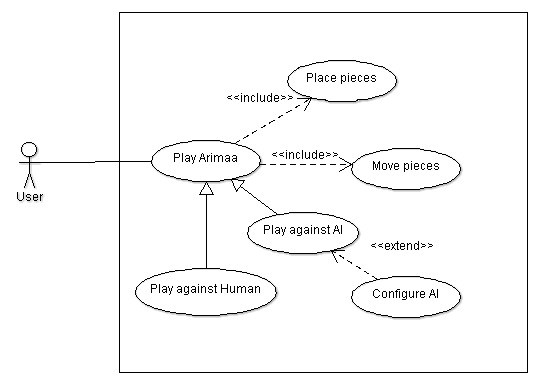
\includegraphics[width=\textwidth]{2General_Architecture/2.1Behaviour_of_the_Game/Pictures/Application_UCD}
\caption{The user-case diagram describing the application}
\label{fig:UCD_Play}
\end{figure}

In order to make the game easy to play, this application will provide a graphical User Interface (further referred to as \emph{UI}). % as described in part ??
This UI, as well as the algorithm for the AI, will act upon the game model, so as to inform it of what moves were made.
The UI will also regularly update to give the player feedback on the progression of the game.

	\subsection{Application-program interface}	\label{sec:api}
	\subsection{Inputs/Outputs}			\label{sec:io}
\newpage

\section{Algorithmic methods}				\label{sec:introduction}
	\subsection{Parallelization methods}		\label{sec:parallelization}
	\subsection{Monte Carlo tree search}		\label{sec:mcts}
\newpage

\section{Software solutions}				\label{sec:introduction}
	\subsection{OpenMP}				\label{sec:openmp}
	\subsection{OpenACC}				\label{sec:openacc}
	\subsection{MPI}					\label{sec:mpi}
\newpage

\section{Conclusion}					\label{sec:conclusion}		
The main focus area of this report is planning. Various planning methods have been decided such as Agile development methodology and Planning Poker method.
Using Agile Development Methodology, the incremental  development of the project will take place. Planning Poker method  which is the estimation technique of Agile Methodology is used to estimate the time requirement for the development of the project. The dates have been estimated with respect to the development of various models of our project.A serious attempt is made analyse the risks  in order to take preventive measures to avoid various risks and problems. 

\newpage

%uncomment to add bibliography
%\bibliography{bibliography}
%\bibliographystyle{plain}

\end{document}
